\section{AIR-TO-AIR GUNNERY}

\subsection{M-61 VULCAN}
\label{subsec:m61}

\begin{figure}[htbp]
    \centering
    \fbox{
    \begin{minipage}[t][40mm][c]{100mm}
        \center{\Large\titlefont\textbf{COMING SOON}}
        % \center{\large\textbf{M-61 OVERVIEW}}
        % \begin{itemize}
        %     \item Some kind of overview figure
        %     \item maybe showing side on profile of the weapon?
        % \end{itemize}
    \end{minipage}
    }
    \caption{M-61 Vulcan}
\end{figure}
% TODO: M61 overview figure!

\begin{tcoloritemize}
    \blueitem{M-61 Vulcan}{
    Internally mounted, high fire-rate, 20mm rotary ``Gattling'' cannon.
    In service since 1959

    \begin{itemize}
        \item \textbf{Fire Rate} --- 6000rpm
        \item \textbf{Round Size} --- 20mm
        \item \textbf{Ammo Capacity} --- 510 rounds
    \end{itemize}}
    \blueitem{Ammunition Types}{
    \begin{itemize}
        \item \textbf{HEI} --- \textbf{H}igh \textbf{E}xplosive \textbf{I}ncendiary
        \item \textbf{HEI-T} --- \textbf{H}igh \textbf{E}xplosive \textbf{I}ncendiary-\textbf{T}racer
        \item \textbf{AP} --- \textbf{A}rmor \textbf{P}iercing
        \item \textbf{TP} --- \textbf{T}arget \textbf{P}ractice
        \item \textbf{SAPHEI} --- \textbf{S}emi \textbf{A}rmor \textbf{P}iercing \textbf{H}igh \textbf{E}xplosive \textbf{I}ncendiary
    \end{itemize}}
    \blueitem{Gunsight / \break Cueing Modes}{
    \begin{itemize}
        \item \textbf{EEGS} --- \textbf{E}nhanced \textbf{E}nvelope \textbf{G}un\textbf{S}ight \\
        \hyperref[subsec:m61:eegssymb]{see \Cref{subsec:m61:eegssymb}}
        \item \textbf{Employment w/o radar track (EEGS level II)} \\
        \hyperref[subsec:m61:eegslvl2]{see \Cref{subsec:m61:eegslvl2}}
        \item \textbf{Employment with radar track (EEGS level V)} \\
        \hyperref[subsec:m61:eegslvl5]{see \Cref{subsec:m61:eegslvl5}}
    \end{itemize}}
    \blueitem{Select GUN}{
    Via Dogfight --- AIM-9 \& GUN automatically selected

    \begin{enumerate}
        \item \textbf{DGFT/MSL OVRD} \dotfill \textbf{DGFT}
    \end{enumerate}

    Via A-A Master Mode

    \begin{enumerate}
        \item \textbf{Master Mode} \dotfill \textbf{A-A}
        \item \textbf{SMS OSB 1} \dotfill \textbf{Cycle to GUN}
    \end{enumerate}}
\end{tcoloritemize}

\subsubsection{SMS CONTROLS}
\label{subsec:m61:sms}
\begin{tcoloritemize}
    \blueitem{Operating Mode}{\textbf{OSB 1} cycles A-A modes, should display \textbf{GUN}}
    \blueitem{Sub-Mode}{\textbf{OSB 2} cycles gunsight modes
    
    \begin{itemize}
        \item \textbf{EEGS} --- \textbf{E}nhanced \textbf{E}nvelope \textbf{G}un\textbf{S}ight \\
        \textbf{see \Cref{subsec:m61:eegssymb}}
    \end{itemize}}
    \blueitem{Rounds \break Remaining}{Indicates number of rounds remaining in 10s}
\end{tcoloritemize}

\begin{figure}[htbp]
    \centering
    \begin{tikzpicture}[auto, node distance=10mm, x=1mm, y=1mm, very thick, line cap=round,
        >={Latex[round]}
        ]
        
        \node[] (fig) at (0,0) {
            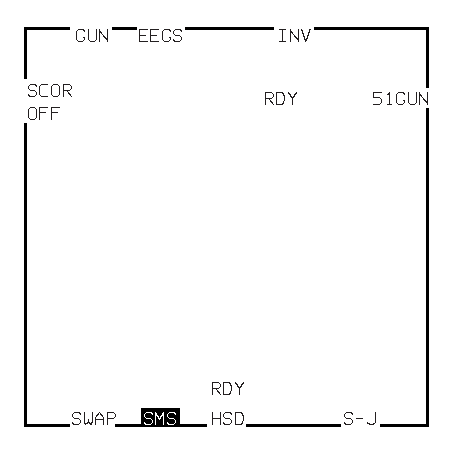
\includegraphics[
                height=75mm,
            ]{mfd/sms/gun.pdf}
        };

        % Annotations
        \node[lannot] (mode) at ($(fig.west)+(0mm,27mm)$) {Operating \\ mode};
        \draw[annotptr] (mode.east) -- ++(10mm, 0mm) -- ++(3mm,3mm);

        \node[lannot] (submode) at ($(fig.west)+(0mm,14mm)$) {Submode};
        \draw[annotptr] (submode.east) -- ++(10mm, 0mm) -- ++(15mm, 15mm);

        \node[rannot] (inv) at ($(fig.east)+(0mm,27mm)$) {Inventory};
        \draw[annotptr] (inv.west) -- ++(-21mm, 0mm) -- ++(-3mm, 3mm);

        \node[rannot] (rounds) at ($(fig.east)+(0mm,14mm)$) {Rounds \\ remaining};
        \draw[annotptr] (rounds.west) -- ++(-4mm,0mm) -- ++(-5mm, 5mm);

        \node[rannot] (rdy) at ($(fig.east)+(0mm,0mm)$) {Ready \\ indication};
        \draw[annotptr] (rdy.west) -- ++(-8mm, 0mm) -- ++(-19mm,19mm);

        \node[rannot] (sj) at ($(fig.east)+(0mm,-22mm)$) {Selective Jettison};
        \draw[annotptr] (sj.west) -- ++(-10mm, 0mm) -- ++(-6mm, -6mm);
    \end{tikzpicture}
    \caption{Gun SMS page}
\end{figure}

\subsubsection{EEGS SYMBOLOGY}
\label{subsec:m61:eegssymb}
\begin{tcoloritemize}
    \blueitem{EEGS}{\textbf{E}nhanced \textbf{E}nvelope \textbf{G}un\textbf{S}ight

    \begin{itemize}
        \item \textbf{Provides multiple levels of symbology depending on presence of radar lock}
    \end{itemize}}
    \blueitem{Level I}{Backup mode displaying only boresight cross in event of INS failure}
    \blueitem{Level II}{Operating mode prior to radar lock

    \begin{itemize}
        \item \textbf{Boresight Cross} --- shows where gun / aircraft is pointed
        \item \textbf{EEGS Funnel}
        \begin{itemize}
            \item displays path of rounds through space
            \item funnel is of set width to judge distance --- adjust width to target wingspan, stabilize edges of funnel on wingtips and fire
        \end{itemize}
        \item \textbf{MGRS} --- \textbf{M}ultiple \textbf{R}eference \textbf{G}un\textbf{S}ight
        \begin{itemize}
            \item 5 line-segments pointing towards boresight
            \item reference for high aspect snap shots (placeing target on MGRS line should have it fly through gun cross)
        \end{itemize}
    \end{itemize}
    
    Reference symbology in \cref{fig:aa_weap:m61:eegslvl2}
    }
    \blueitem{Level III / IV}{Intermediate modes during radar lock acquisition}
    \blueitem{Level V}{Operating mode with radar lock. Level II symbology is retained with additional elements
    
    \begin{itemize}
        \item \textbf{Level V Pipper}
        \begin{itemize}
            \item gunfire solution --- stabilize pipper on target and fire
            \item contains additional range/aspect cues
        \end{itemize}
        \textbf{reference \cref{fig:aa_weap:m61:eegslvl5,fig:aa_weap:m61:eegs:5pipper}}
        \item \textbf{T-Symbol}
        \begin{itemize}
            \item \textbf{``--- + ---'' 1G Pipper} --- lead angle for non-maneuvering target,
            flanking horizontal lines indicate out-of-plane maneuver potential of target
            \item \textbf{``---'' Max-G Pipper} --- lead angle for target pulling max-G towards you
        \end{itemize}
        \textbf{reference \cref{fig:aa_weap:m61:eegs:tsymb}}
        \item \textbf{Range Caret}
        \begin{itemize}
            \item displayed on \underline{inside} edge of level V pipper
            \item unwinds from 12 o'clock at 12'000ft counter-clockwise
        \end{itemize}
        \textbf{reference \cref{fig:aa_weap:m61:eegs:tdescirc}}
        \item \textbf{Aspect Caret} 
        \begin{itemize}
            \item displayed on \underline{outside} edge of level V pipper
        \end{itemize}
        \textbf{reference \cref{fig:aa_weap:m61:eegs:tdescirc}}
        \item \textbf{BATR} --- \textbf{B}ullets \textbf{A}t \textbf{T}arget \textbf{R}ange
        \begin{itemize}
            \item displayed once rounds have been fired
            \item dissappears after last round has passed beyond target range
            \item useful to evaluate shots (also for training)
        \end{itemize}
        \textbf{reference \cref{fig:aa_weap:m61:eegs:pipper}}
    \end{itemize}
    
    Reference symbology in \cref{fig:aa_weap:m61:eegslvl5,fig:aa_weap:m61:eegs:5pipper}
    }
\end{tcoloritemize}

\begin{figure}[htbp]
    \centering

    \begin{tikzpicture}[auto, node distance=10mm, x=1mm, y=1mm, very thick, line cap=round,
        >={Latex[round]}
        ]
        
        \node[draw, rounded corners] (fig) at (0,0) {
            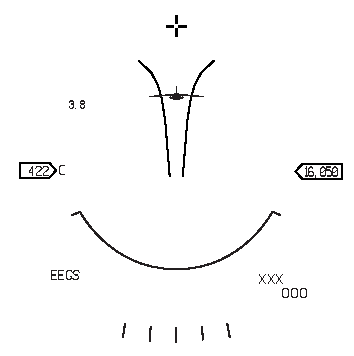
\includegraphics[
                height=75mm,
            ]{hud/eegs/lvl2.pdf}
        };

        % Annotations
        \node[lannot] (boresight) at ($(fig.west)+(-2.5mm,32mm)$) {Boresight cross};
        \draw[annotptr] (boresight.east) -- (-5mm,32mm);

        \node[rannot] (bandit) at ($(fig.east)+(2.5mm,12mm)$) {Bandit};
        \draw[annotptr] (bandit.west) -- ++(-36mm, 0mm) -- ++(-4mm,4mm);

        \node[lannot] (funnel) at ($(fig.west)+(-2.5mm,12mm)$) {EEGS Funnel};
        \draw[annotptr] (funnel.east) -- (-5mm,12mm);

        \node[lannot] (mgrs) at ($(fig.west)+(-2.5mm,-32mm)$) {MGRS Lines};
        \draw[annotptr] (mgrs.east) -- (-15mm,-32mm);
    \end{tikzpicture}
    \caption{EEGS LVL II HUD Symbology}
    \label{fig:aa_weap:m61:eegslvl2}
\end{figure}

\begin{figure}[htbp]
    \centering

    \begin{tikzpicture}[auto, node distance=10mm, x=1mm, y=1mm, very thick, line cap=round,
        >={Latex[round]}
        ]
        
        \node[draw, rounded corners] (fig) at (0,0) {
            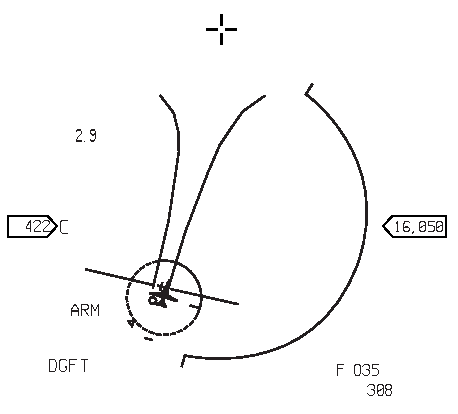
\includegraphics[
                height=75mm,
            ]{hud/eegs/lvl5.pdf}
        };

        % Annotations
        \node[lannot] (boresight) at ($(fig.west)+(-2.5mm,32.25mm)$) {Boresight cross};
        \draw[annotptr] (boresight.east) -- (-7mm,32.25mm);

        \node[lannot] (funnel) at ($(fig.west)+(-2.5mm,8mm)$) {EEGS Funnel};
        \draw[annotptr] (funnel.east) -- (-12mm,8mm);

        \node[rannot] (bandit) at ($(fig.east)+(2.5mm,-16mm)$) {Bandit};
        \draw[annotptr] (bandit.west) -- ++(-37mm, 0mm) -- (-9mm,-16mm);

        \node[lannot] (pipper) at ($(fig.west)+(-2.5mm,-16mm)$) {EEGS Level V Pipper};
        \draw[annotptr] (pipper.east) -- (-20mm,-16mm);
    \end{tikzpicture}
    \caption{EEGS LVL V HUD Symbology}
    \label{fig:aa_weap:m61:eegslvl5}
\end{figure}

\begin{figure}[htbp]
    \centering
    \begin{subfigure}[b]{\linewidth}
        \centering
        \begin{tikzpicture}[figstyle]

            \node[draw, rounded corners] (fig) at (0,0) {
                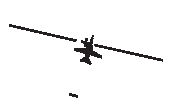
\includegraphics[
                    scale=1.75,
                ]{hud/eegs/lvl5_subfig_tsymb.pdf}
            };

            % Annotations
            \node[lannot] (1g) at ($(fig.west)+(-2.5mm,12mm)$) {1-g Pipper};
            \draw[annotptr] (1g.east) -- ++(22mm,0mm) -- ++(6mm,-6mm);

            \node[lannot] (9g) at ($(fig.west)+(-2.5mm,-12mm)$) {9-g Pipper};
            \draw[annotptr] (9g.east) -- ++(22mm,0mm);

            \node[rannot] (manpot) at ($(fig.east)+(2.5mm,5mm)$) {Maneuver potential lines};
            \draw[annotptr] (manpot.west) -- ++(-10mm, 0mm) -- ++(-4mm,-4mm);

        \end{tikzpicture}
        \caption{T-symbol}
        \label{fig:aa_weap:m61:eegs:tsymb}
    \end{subfigure}

    \vspace{2em}
    \begin{subfigure}[b]{\linewidth}
        \centering
        \begin{tikzpicture}[figstyle]

            \node[draw, rounded corners] (fig) at (0,0) {
                
\includegraphics[
                    scale=1.75,
                ]{hud/eegs/lvl5_subfig_tdcircle.pdf}
            };

            % Annotations
            \node[lannot] (12oclock) at ($(fig.west)+(-2.5mm,13mm)$) {12000 ft};
            \draw[annotptr] (12oclock.east) -- ++(14mm,0mm) -- ($(fig.north) + (-2mm,-3mm)$);

            \node[lannot] (9oclock) at ($(fig.west)+(-2.5mm,0mm)$) {9000 ft};
            \draw[annotptr] (9oclock.east) -- ++(6mm,0mm);

            \node[lannot] (aspect) at ($(fig.west)+(-2.5mm,-10mm)$) {Aspect caret};
            \draw[annotptr] (aspect.east) -- ++(4mm,0mm) -- (-11mm, -8.5mm);

            \node[rannot] (rcue) at ($(fig.east)+(2.5mm,8mm)$) {Range cue};
            \draw[annotptr] (rcue.west) -- ++(-8mm, 0mm) -- (8.5mm,-1mm);

            \node[rannot] (3oclock) at ($(fig.east)+(2.5mm,0mm)$) {3000 ft};
            \draw[annotptr] (3oclock.west) -- ++(-6mm,0mm);

            \node[rannot] (6oclock) at ($(fig.east)+(2.5mm,-13mm)$) {6000 ft};
            \draw[annotptr] (6oclock.west) -- ++(-14mm,0mm) -- ($(fig.south) + (2mm,3mm)$);

        \end{tikzpicture}
        \caption{target designator circle}
        \label{fig:aa_weap:m61:eegs:tdescirc}
    \end{subfigure}

    \vspace{2em}
    \begin{subfigure}[b]{\linewidth}
        \centering
        \begin{tikzpicture}[figstyle]

            \node[draw, rounded corners] (fig) at (0,0) {
                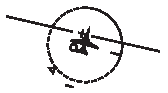
\includegraphics[
                    scale=1.75,
                ]{hud/eegs/lvl5_subfig_full.pdf}
            };

            % Annotations
            \node[lannot] (batr) at ($(fig.west)+(-2.5mm,0mm)$) {BATR \\ circle};
            \draw[annotptr] (batr.east) -- ++(23mm,0mm);

            \node[rannot] (bandit) at ($(fig.east)+(2.5mm,-6mm)$) {Bandit};
            \draw[annotptr] (bandit.west) -- ++(-22mm,0mm) -- ++(-4mm, 4mm);
        \end{tikzpicture}
        \caption{full, combined pipper, shown approx. on-target}
        \label{fig:aa_weap:m61:eegs:pipper}
    \end{subfigure}
    \caption{EEGS Level V Pipper, split by component}
    \label{fig:aa_weap:m61:eegs:5pipper}
\end{figure}

\marginfigeometry

\subsubsection{GUN SELECTION}
\label{subsec:m61:selection}
\begin{checklistitemize}
    \blueitem{Via Dogfight}{(GUN automatically selected)
    \begin{enumerate}
        \item \textbf{DGFT/MSL OVRD} \dotfill \textbf{DGFT}
    \end{enumerate}}
    \blueitem{Via A-A Master Mode}{
    \begin{enumerate}
        \item \textbf{Master Mode} \dotfill \textbf{A-A}
        \item \textbf{SMS OSB 1} \dotfill \textbf{Cycle to GUN}
    \end{enumerate}}
    \blueitem{EEGS Symbology}{Verify
    \begin{itemize}
        \item \textbf{EEGS Level II} appears if no lock present
        \item \textbf{EEGS Level V} appears if target locked
    \end{itemize}}
\end{checklistitemize}

\subsubsection{EEGS LVL II EMPLOYMENT --- NO RADAR}
\label{subsec:m61:eegslvl2}
\begin{checklistenumerate}
    \blueitem{Prerequisites}{
    \begin{itemize}
        \item \textbf{RF Switch} \dotfill \textbf{SILENT} \\
        \hfill (if desired, completely silences radar)
        \item \textbf{Selected Weapon} \dotfill \textbf{GUN}
        \item \textbf{Master Arm} \dotfill \textbf{ARM}
    \end{itemize}}
    \blueitem{Acquire Firing Solution}{
    \marginpar{
        \captionsetup{type=figure}
        \centering
        \begin{tikzpicture}[figstyle]
            
            \node[boxedmarfigstyle] (fig) at (0,0) {
                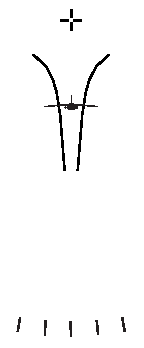
\includegraphics[
                    scale=1.25,
                ]{hud/eegs/lvl2_subfig_funnel_mgrs.pdf}
            };
        \end{tikzpicture}
        \caption{EEGS Funnel \& MGRS Lines. Target is approx. aligned with funnel.}
    }

    \smallskip
    Using EEGS funnel

    \begin{enumerate}
        \item \textbf{EEGS Funnel} \dotfill \textbf{Stabilized On-Target}
        \item \textbf{Funnel Lines} \dotfill \textbf{On target wingtips}
    \end{enumerate}

    Using MGRS lines
    
    \begin{enumerate}
        \item \textbf{MGRS Line} \dotfill \textbf{Aligned with target}
    \end{enumerate}}
    \blueitem{Fire Gun}{
    \begin{enumerate}
        \item \textbf{TRIGGER} \dotfill \textbf{2nd Detent}
        \item Adjust lead to achieve desired effects
    \end{enumerate}}
\end{checklistenumerate}

% \notebox{
%     \small
%     \textbf{Exact position of target relative to funnel lines dependent on funnel width and target wingspan, 
%     see \Cref{subsec:m61:eegsfunneladjust} for funnel adjustment.}
% }

\marnotebox{
    \footnotesize
    \textbf{Exact position of target relative to funnel lines dependent on funnel width and target wingspan}
}

\clearpage

\subsubsection{EEGS LVL V EMPLOYMENT --- RADAR}
\label{subsec:m61:eegslvl5}
\begin{checklistenumerate}
    \blueitem{Prerequisites}{
    \begin{itemize}
        \item \textbf{FCR Switch} \dotfill \textbf{FCR}
        \item \textbf{RF Switch} \dotfill \textbf{NORM}
        \item \textbf{Selected Weapon} \dotfill \textbf{GUN}
        \item \textbf{Master Arm} \dotfill \textbf{ARM}
    \end{itemize}}
    \blueitem{Radar Acquisition}{ACM selected automatically in \textbf{DGFT} mode, \textbf{see \Cref{subsec:acm}}

    \begin{enumerate}
        \item \textbf{ACM Submode} \dotfill \textbf{As desired}
        \item Maneuver to place target in radar scan volume
    \end{enumerate}}
    \blueitem{Acquire Firing Solution}{
    \marginpar{
        \captionsetup{type=figure}
        \centering
        \begin{tikzpicture}[figstyle]
            \node[boxedmarfigstyle] (fig) at (0,0) {
                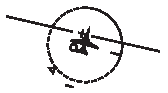
\includegraphics[
                    scale=1.25,
                ]{hud/eegs/lvl5_subfig_full.pdf}
            };
        \end{tikzpicture}
        \caption{EEGS Level V Pipper}
    }
    \begin{enumerate}
        \item \textbf{Pipper} \dotfill \textbf{Stabilized On-Target}
    \end{enumerate}}
    \blueitem{Fire Gun}{
    \begin{enumerate}
        \item \textbf{TRIGGER} \dotfill \textbf{2nd Detent}
        \item Adjust lead to achieve desired effects
    \end{enumerate}}
\end{checklistenumerate}

\subsubsection{ADJUST EEGS FUNNEL WIDTH}
\label{subsec:m61:eegsfunneladjust}
\begin{checklistenumerate}
    \blueitem{Open DED MAN Page}{
    \begin{enumerate}
        \item \textbf{ICP LIST Button} \dotfill \textbf{Press}
        \item \textbf{DED MAN Page} \dotfill \textbf{Open (5)} 
    \end{enumerate}}
    \blueitem{Adjust Wingspan}{
    \begin{enumerate}
        \item \textbf{WSPAN} \dotfill \textbf{Selected}
        \item \textbf{Desired Value} \dotfill Input on ICP, \textbf{ENTR}
        \item \textbf{WSPAN} \dotfill Verify as desired
    \end{enumerate}}
\end{checklistenumerate}

\marginfigrestore